\chapter{Evaluation}

In this section, the proposed optimal control approach is implemented and its effectiveness tested and compared to the previous approach. The simulation setup is described in Sec. \ref{setup} and the results are shown in Sec. \ref{optimal control}. Sec. \ref{computation time} and Sec. \ref{performance guarantees} then focuses on the general performance of this new method in comparison to the previously used Scenario approach.

\section{Setup} \label{setup}

\section{Optimal Control with known basis functions} \label{optimal control}

\begin{figure}[htb]
\centering
\subfigure[Scenario Approach]{
   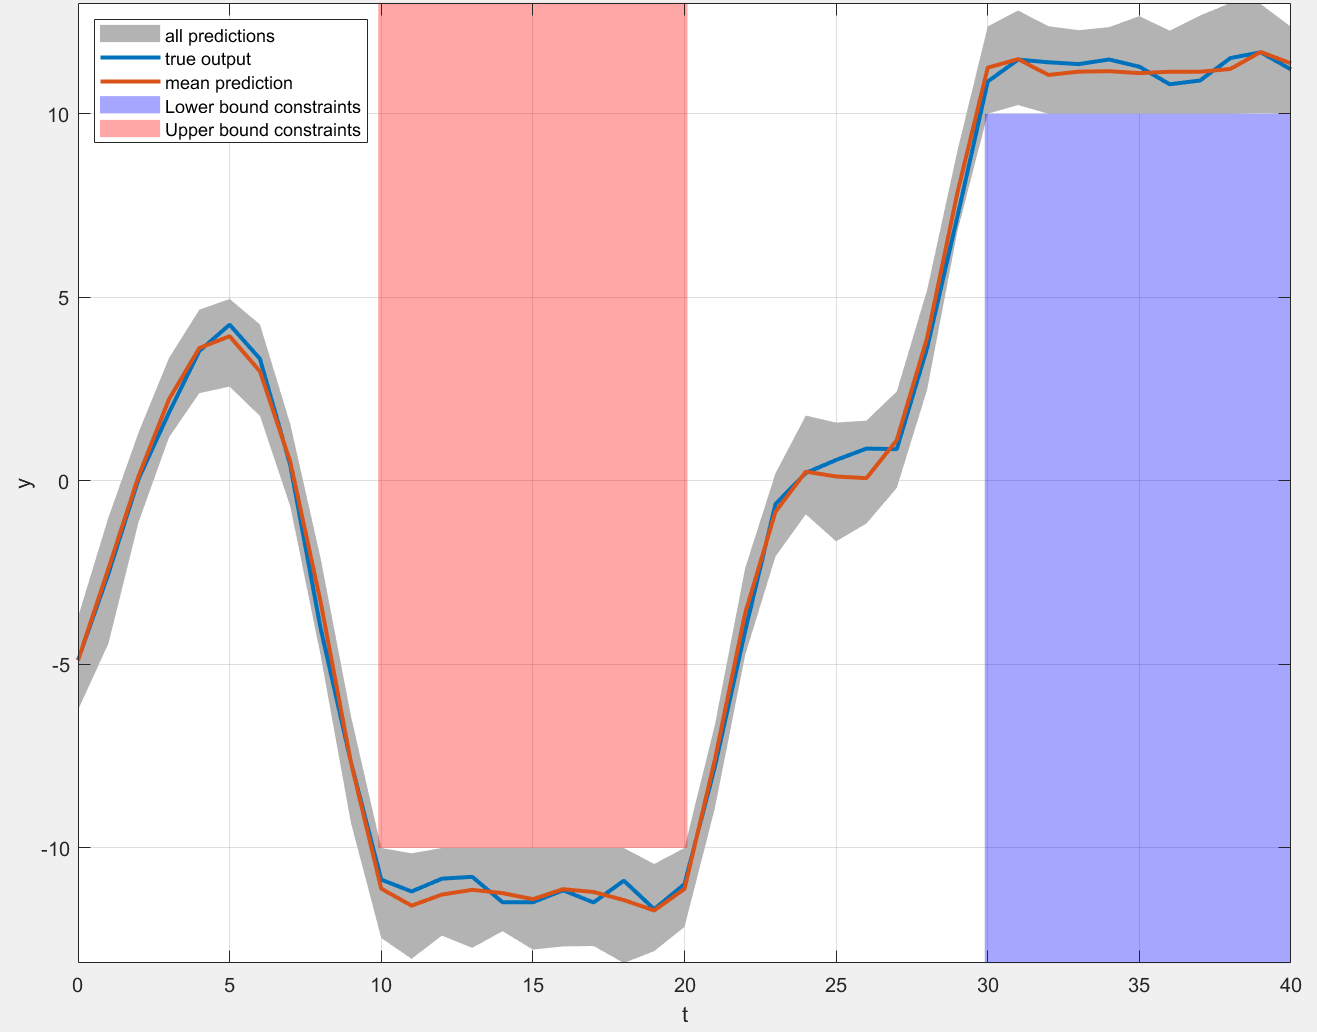
\includegraphics[width=0.4\textwidth] {pics/Scenario_plot.png}
   \label{fig:subfig1}
 }
\quad % puts next subfigure right next to the previous subfigure
\subfigure[Kernel Approach]{
   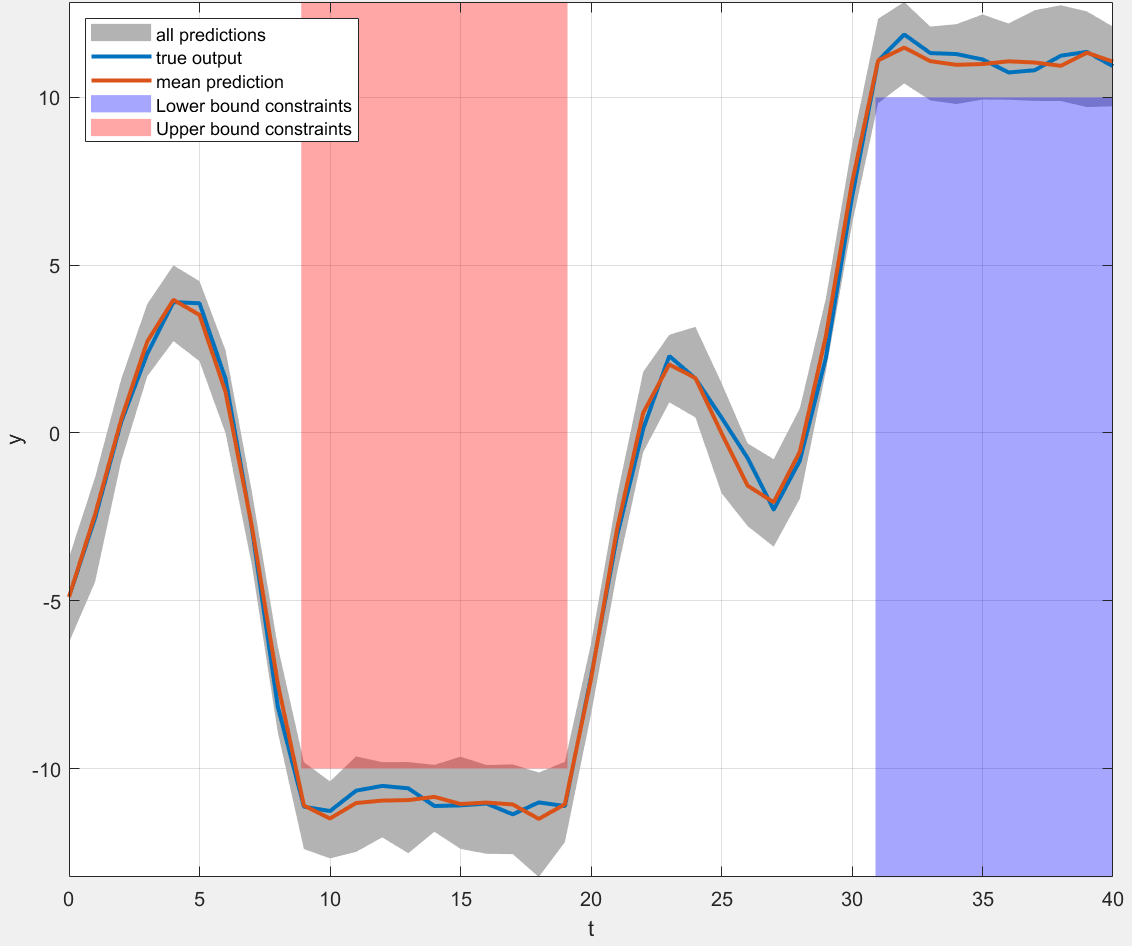
\includegraphics[width=0.4\textwidth] {pics/Kernel_plot.png}
   \label{fig:subfig2}
 }
\caption{Example of the optimal control with known basis functions for scenario approach (left) and kernel approach (right). The red and blue area show the output constraints. The gray area encompasses the 200 scenarios that were used in the optimization with the orange line being the average. The blue line is one realization the true output.}
\end{figure}

\section{Robustness} \label{performance guarantees}

The biggest advantage that this kernel approximation proves compared to the scenario approach is the adjustable robustness of the solution. As described in Sec. \ref{Sec:CCOKernel}, this method includes a parameter $\alpha \in [0, 1]$ which can be chosen depending on how robust the final solution is supposed to be. 

In this section, this parameter is tested by running the same problem setup as was used in Sec. \ref{optimal control} for different values of $\alpha$ as well as an increasing number of samples $N$ and testing how well the solution holds up for future scenarios.

Similar to Sec. \ref{optimal control}, $N = 200$ scenarios are generated with Algorithm \ref{alg:PGibbs}. From this set of 200 scenarios, a small subset is then taken and used to formulate several OCPs as was already described in Sec. \ref{optimal control}. The OCPs are then solved and the resulting optimal input $\boldsymbol{u}_{0:H}$ is then used on $N = 2000$ more scenarios to estimate the robustness of the solution. For each of the 2000 scenarios, the output is calculated and compared to the constraints that were used in the OCP. This process is then repeated over and over for a slightly larger subset of scenarios until finally the full set of $N = 200$ scenarios is used.

\begin{figure}[htb]
\centering
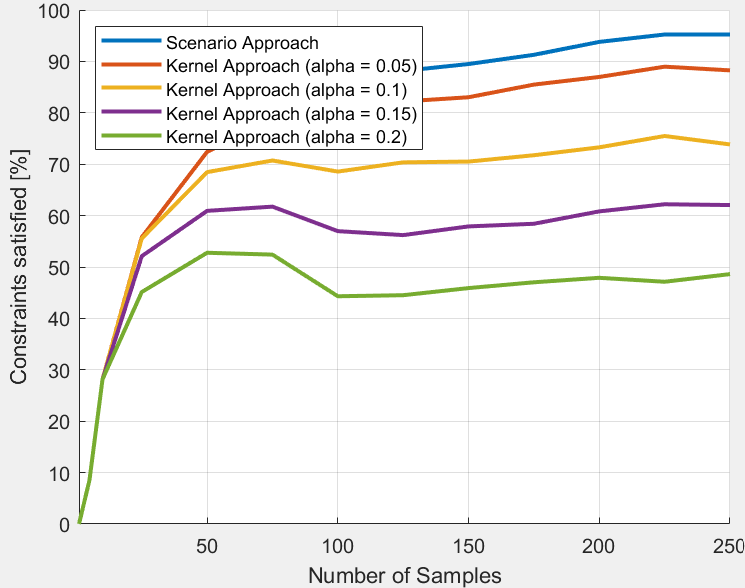
\includegraphics[width=0.7\textwidth]{pics/robustness_plot.png}
\caption{Estimated Robustness of solution $\boldsymbol{u}$ over number of samples $N$. The blue line shows the result of the scenario approach while the other lines are for the Kernel approach with various values of $\alpha$}
\label{fig:robustness_plot}
\end{figure}

In Fig. \ref{fig:robustness_plot} the results of this simulation are shown. The percentage of scenarios that fulfill the constraints is plotted over the number of samples used in the initial optimization which range from $N = 1$ to 200. The various $\alpha$ values are shown as separate lines. Initially, all five plots show very robustness. This can be explained by the fact that at such a low number of scenarios cannot accurately represent the distribution. As the number of scenarios is increased, the approximation of the distribution becomes better as well and the solution of the OCP now represents a larger number of the distribution. 

After around 10 scenarios, the plots start diverging for the first time. While the scenario approach and the plots with smaller $\alpha$ values are very similar, the lines that represent larger $\alpha$ values are starting to display worse robustness. This trend continues as the number of scenarios used in the optimization keeps increasing. While the scenario approach keeps increasing, the Kernel approach seems to converge to a significantly lower level of robustness based on the selection of the parameter $\alpha$. This shows that the robustness can be somewhat controlled with the parameter $\alpha$.

 

\section{Computation Time} \label{computation time}

While the previous sections focused on comparing the results of the Scenario approach to the kernel approach, the runtime of both methods is another important factor that needs to be considered when choosing which algorithm is best suited for a specific problem. As such, Fig. \ref{fig:runtime_plot} shows the runtime of both scenario approach and kernel approach over the number of scenarios that are used to formulate the OCPs. The parameters and constraints are chosen the same as in Sec. \ref{optimal control}. When looking at the figure, it quickly becomes apparent that while both curves start around the same level, the kernel approach runtime increases significantly faster and with more of a curvature than the scenario approach. By the end of the plot, the kernel approach already takes about 5 times as long as the scenario approach. This shows that at least when it comes to finding a solution quickly, the Scenario approach is still the better choice.

\begin{figure}[htb]
\centering
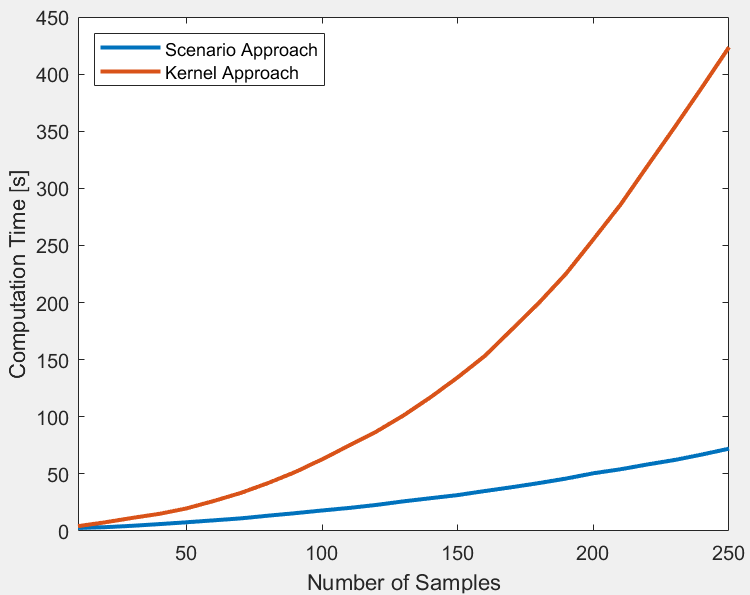
\includegraphics[width=0.6\textwidth]{pics/computationtime_plot.png}
\caption{Runtime over number of samples $N$ for scenario and kernel approach}
\label{fig:runtime_plot}
\end{figure}
